\documentclass[border=1cm,10pt]{standalone}

% I only need the arrows for this one.
\usepackage{tikz}
\usetikzlibrary{arrows}
\usetikzlibrary{decorations.pathmorphing}
\usetikzlibrary{decorations.markings}
\usetikzlibrary{trees}

\begin{document}

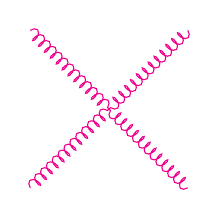
\begin{tikzpicture}[
  boson/.style={decorate, decoration={snake}, draw=red},
  lepton/.style={draw=blue, postaction={decorate},
        decoration={markings,mark=at position .55 with {\arrow[draw=blue]{>}}}},
  alepton/.style={draw=blue, postaction={decorate},
        decoration={markings,mark=at position .55 with {\arrow[draw=blue]{<}}}},
  quark/.style={draw=black, postaction={decorate},
        decoration={markings,mark=at position .55 with {\arrow[draw=black]{>}}}},
  aquark/.style={draw=black, postaction={decorate},
        decoration={markings,mark=at position .55 with {\arrow[draw=black]{<}}}},
  gluon/.style={decorate, draw=magenta, decoration={coil,amplitude=2pt, segment length=3pt}} 
]

% Draw the boson
\draw[gluon] (0,0) -- (1,1)  ;
\draw[gluon] (2,0) -- (1,1)  ;
\draw[gluon] (2,2) -- (1,1)  ;
\draw[gluon] (0,2) -- (1,1)  ;

\end{tikzpicture}

\end{document} 
